\subsection{Molle e Forza Elastica}
\begin{center}
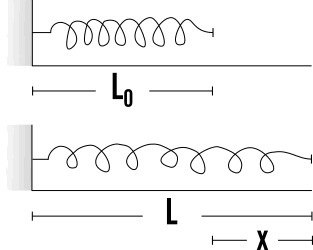
\includegraphics[width=0.4 \linewidth]{Dinamica/forza-elastica.png} 
\end{center}
\begin{gather*}
    \text{Lunghezza della molla a riposo: } L_0 \\
    \text{Elongazione: } x = L - L_0 \\
    \text{Legge di Hooke(Forza Elastica): } F_e = -k x
\end{gather*}